\section{Literature Review}
This section represents a brief relevant literature on the Flexible Job Shop Scheduling Problem (FJSSP), which was initially used as a general scheduling model for semiconductor production. Alternatively, this moves on with a discussion around the Semiconductor Manufacturing Scheduling Problem (SMSP), and how it can proceed with Ant Colony Optimization (ACO) and the solution.
\subsection{Semiconductor Manufacturing Scheduling Problem (SMSP)}
The SMSP is a complex and critical challenge to optimize scheduling tasks during the manufacturing process of a semiconductor. Different methods have been adopted for a long time for varied types of machines \cite{chan2024situation}. The core aspects include job scheduling, batch processing, priority constraints, setup times of the machine, machine availability, and reentrant flow. The key challenges stay with complexity, dynamic job arrivals, and reducing downtime while maximizing throughput \cite{el2023hybrid}. Many researchers and developers have been working on the topic and suggested their methods to solve the problem.
\vspace{1em}

Mixed-integer linear programming (MILP) is a great option to solve large mathematical problems by optimizing the solution. As suggested by \cite{fang2023problems} in their study to identify important research problems with semiconductor manufacturing operations (SMOs), MILP models are extensively used in deterministic SMO scheduling problems. While MILP models are great for optimal solutions for small-scale instances, these models can also be used to provide upper bounds for large-scale instances. The only thing is, there is no optimal solution for such situations, but it is done by relaxing several constraints. 
\vspace{1em}

Another paper \cite{wang2014hybrid} was written for research of an SMSP to solve all the constraints of the semiconductor manufacturing industry such as machine status, setup time, limited waiting time, different process times on varied machines, and more. The researchers suggested a hybrid estimation of a distribution algorithm with multiple subpopulations (HEDA-MS) to solve SMSP and to make the total exceed the limited waiting time to zero.
\subsection{Flexible Job Shop Scheduling}
Considering the manufacturing industry, FJSSP is a common problem, especially for small batch and custom productions. The mathematical models allow us to solve the optimality issue for small-scale instances. As \cite{dauzere2024flexible} explains in their paper, it is important to assign the FJSSP on a machine in a particular sequence. As the optimization criteria need the start time of all the operations, it is important to optimize the completion time also. The most suitable approach to solve this time problem depends on the function and the mathematical properties associated with it. Researchers also explained that many studies are optimizing non-regular criteria that require equal efforts for timing decisions to get the best sequencing decisions in solution approaches. 
\vspace{1em}

\begin{figure}[ht]
  \centering
  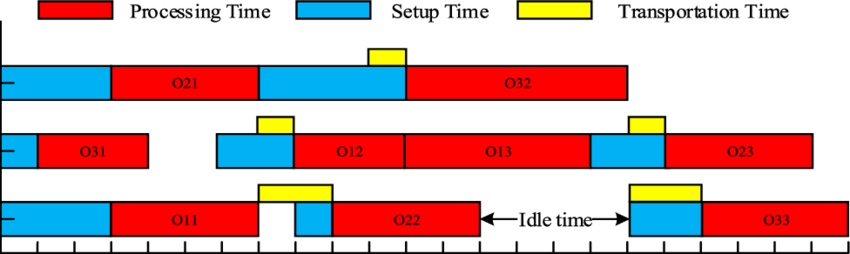
\includegraphics[width=0.5\textwidth]{FJSSP.png} 
  \caption{Example of the flexible job-shop scheduling problem \cite{zhang2022novel}}
  \label{fig:image2}
\end{figure}

\vspace{1em}
The study \cite{lei2022multi} explained that the existing methods to solve NP-hard combinatorial optimization problems are either exact or approximate. The exact methods are challenging to solve FJSSP when problems need large-size scheduling. Considering their NP-hardness, it is difficult to allocate reasonable time. \cite{lei2022multi} have also explained that FJSSP instances intractability is in constant need of more approximate methods. So many solutions like machine learning techniques, heuristics, meta-heuristics methods, and more are continuously being developed to tackle real-world problems more effectively. 

\vspace{1em}
In their recent work, \cite{zhang2020evolving} used generic programming to evolve scheduling heuristics in dynamic FJSS. They explained that Genetic programming hyperheuristics (GPHH) is a great option for heuristics scheduling, and a proper selection of the terminal makes it successful. They concluded that a two-stage GPHH with selected features for DFJSS can help in interpretable scheduling heuristics while creating a much shorter training time.
\subsection{Ant Colony Optimization}
ACO follows the foraging methods of ant species to find a favorable path and leaves the trails (pheromone) to let others find the path. ACO algorithms are one of the MPPT methods to search for GMPP. Sometimes it is also used as a hybrid MPPT method \cite{mamur2022future}. 
\vspace{1em}

\begin{figure}[ht]
  \centering
  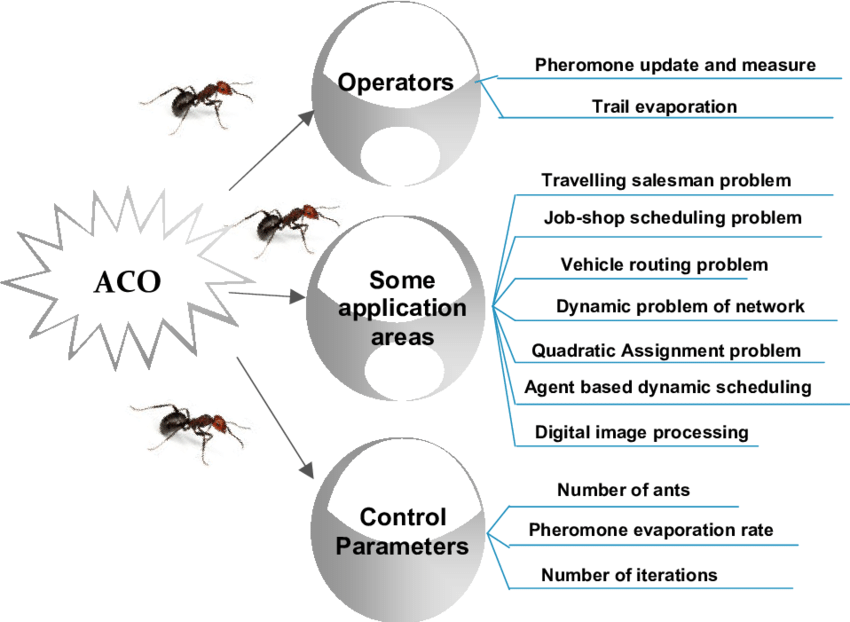
\includegraphics[width=0.5\textwidth]{ACO.png} 
  \caption{Ant Colony Optimization Algorithm working for scheduling \cite{rajan2015investigation}}
  \label{fig:image1}
\end{figure}

\vspace{1em}
ACO is a well-suited metaheuristics algorithm to solve SMSP as it is highly appropriate to handle the dynamic and complex nature of semiconductor scheduling with its multi-objective nature \cite{nayar2021ant}. ACO has a history of application to be applied to SMSP for wafer scheduling to balance the load and minimize the makespan. The dynamic nature of the ACO algorithm continuously updates the “pheromone” based on the completed jobs, and guides others to follow the optimal scheduling decisions, ultimately making the system reduce their decision-making time \cite{zhou2022parameter}.
\vspace{1em}
In their work, \cite{li2024modified} proposed an Ant Colony Algorithm (ACA) to solve constraints like holding times and time lags. They created this setup in two stages where they located pheromones in the first stage while using genetic algorithms to initialize. \cite{shao2010minimising} used the ACO algorithm to form batches. They batched using a DP algorithm and combined it with the job sequences generated by the ACO algorithm that released time to update pheromone trails. 
\vspace{1em}
ACO has been a promising algorithm for FJSSP solving. Researchers didn’t stop there but created extended versions of ACOs to improve time-span minimization. \cite{skackauskas2022dynamic} proposed Dynamic Impact, an extended method for ACO that improved convergence and optimized problems between the resources having non-linear relationships. \cite{skackauskas2022dynamic} concluded a 33.2 percent improved optimization over ACO with the Dynamic Impact algorithm. 
\vspace{1em}
\cite{wang2021time} has explained the importance of improved ACO to ensure real-time determination as a time-sensitive network (TSN). This improved ACO (IACO) focuses on convergence speed and schedules the time-triggered flows in TSN.
%\printbibliography % This will print the bibliography

